\documentclass{beamer}

\usetheme{polimi}
% Usage instructions can be found at: https://github.com/elauksap/beamerthemepolimi

\usepackage[utf8]{inputenc}
\usepackage{graphicx}
\usepackage{booktabs}


\title{NAML Project}
\subtitle{Classify musical genre using audio files}
\author{Peng, Rao}
\date{\today}

\begin{document}

\begin{frame}
  \maketitle
\end{frame}

\begin{frame}{Table of contents}
  \tableofcontents
\end{frame}

\section{Introduction}
% Section page.
\begin{frame}{}
  This project presents multiple machine learning models and Convolutional Neural Networks to classify music genres using audio files.
\end{frame}

\section{Data Exploration}
\begin{frame}{Data Exploration}
  \begin{itemize}
    \item The GTZAN dataset contains 1000 audio tracks from 10 different genres.
    \item The dataset is divided into 10 folders, each containing 100 audio tracks from a specific genre.
    \item The audio tracks are in .wav format and have a sample rate of 22050 Hz.
  \end{itemize}
\end{frame}

\begin{frame}{Waveform}

  \begin{figure}
    \centering
    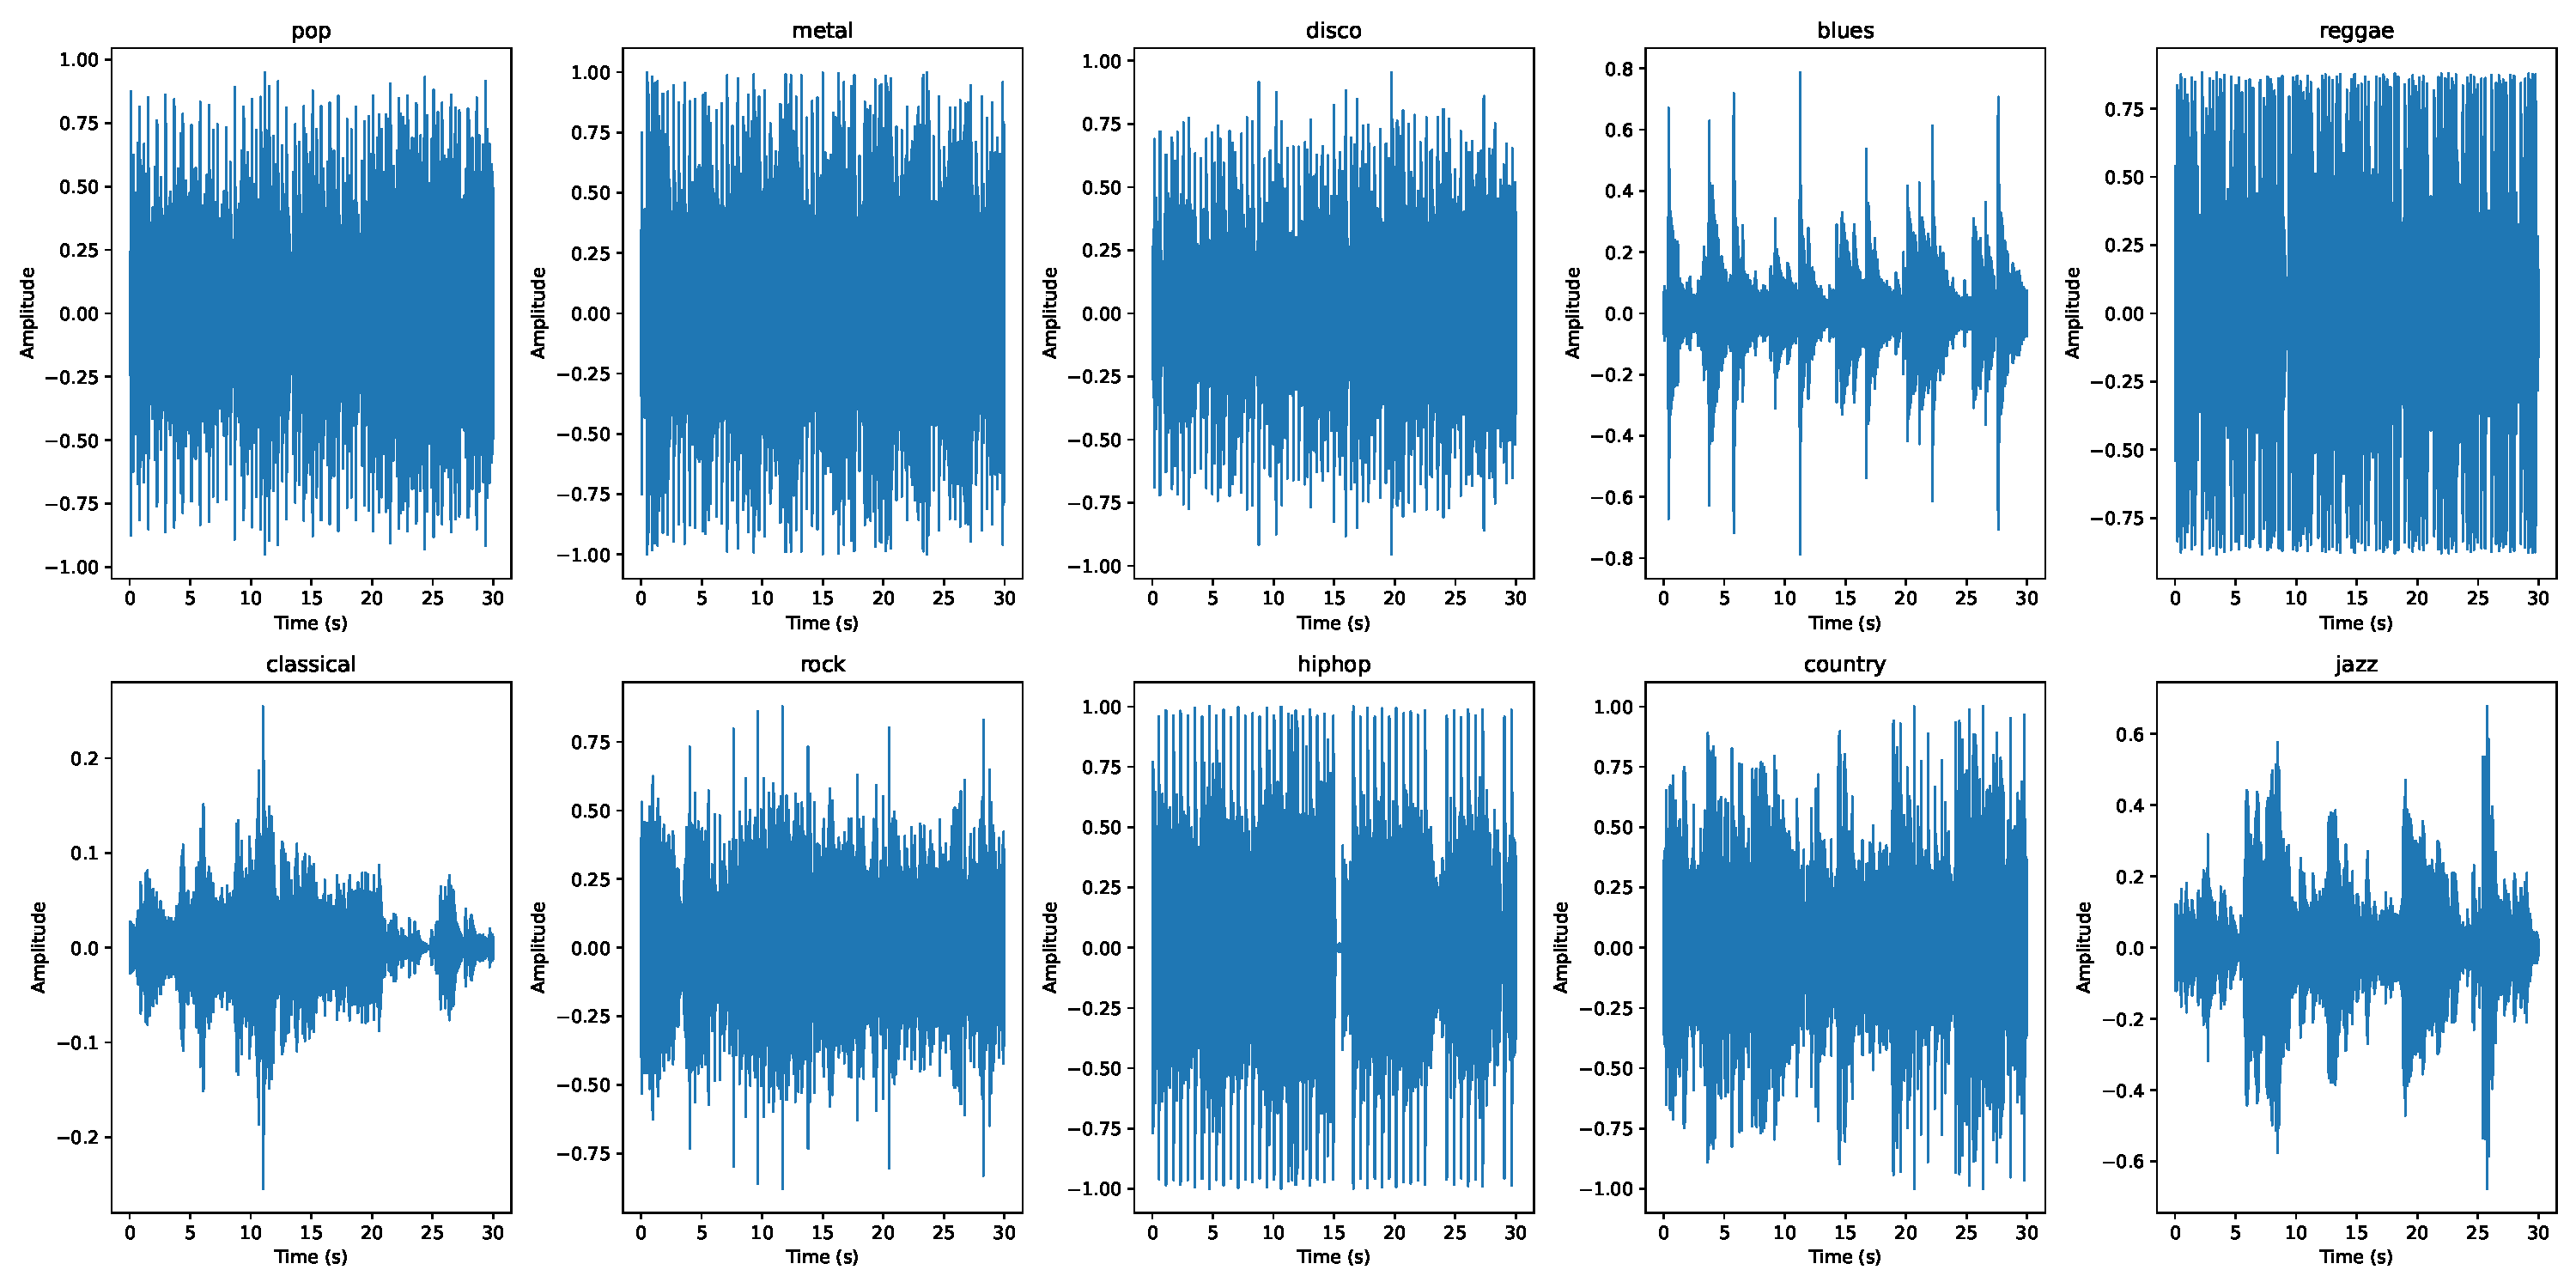
\includegraphics[width=0.9\textwidth]{images/waveform.pdf}
    \caption{Waveform of various sample audios track over time}
    \label{fig:waveform}
  \end{figure}
\end{frame}

\begin{frame}{Chroma}

  \begin{figure}
    \centering
    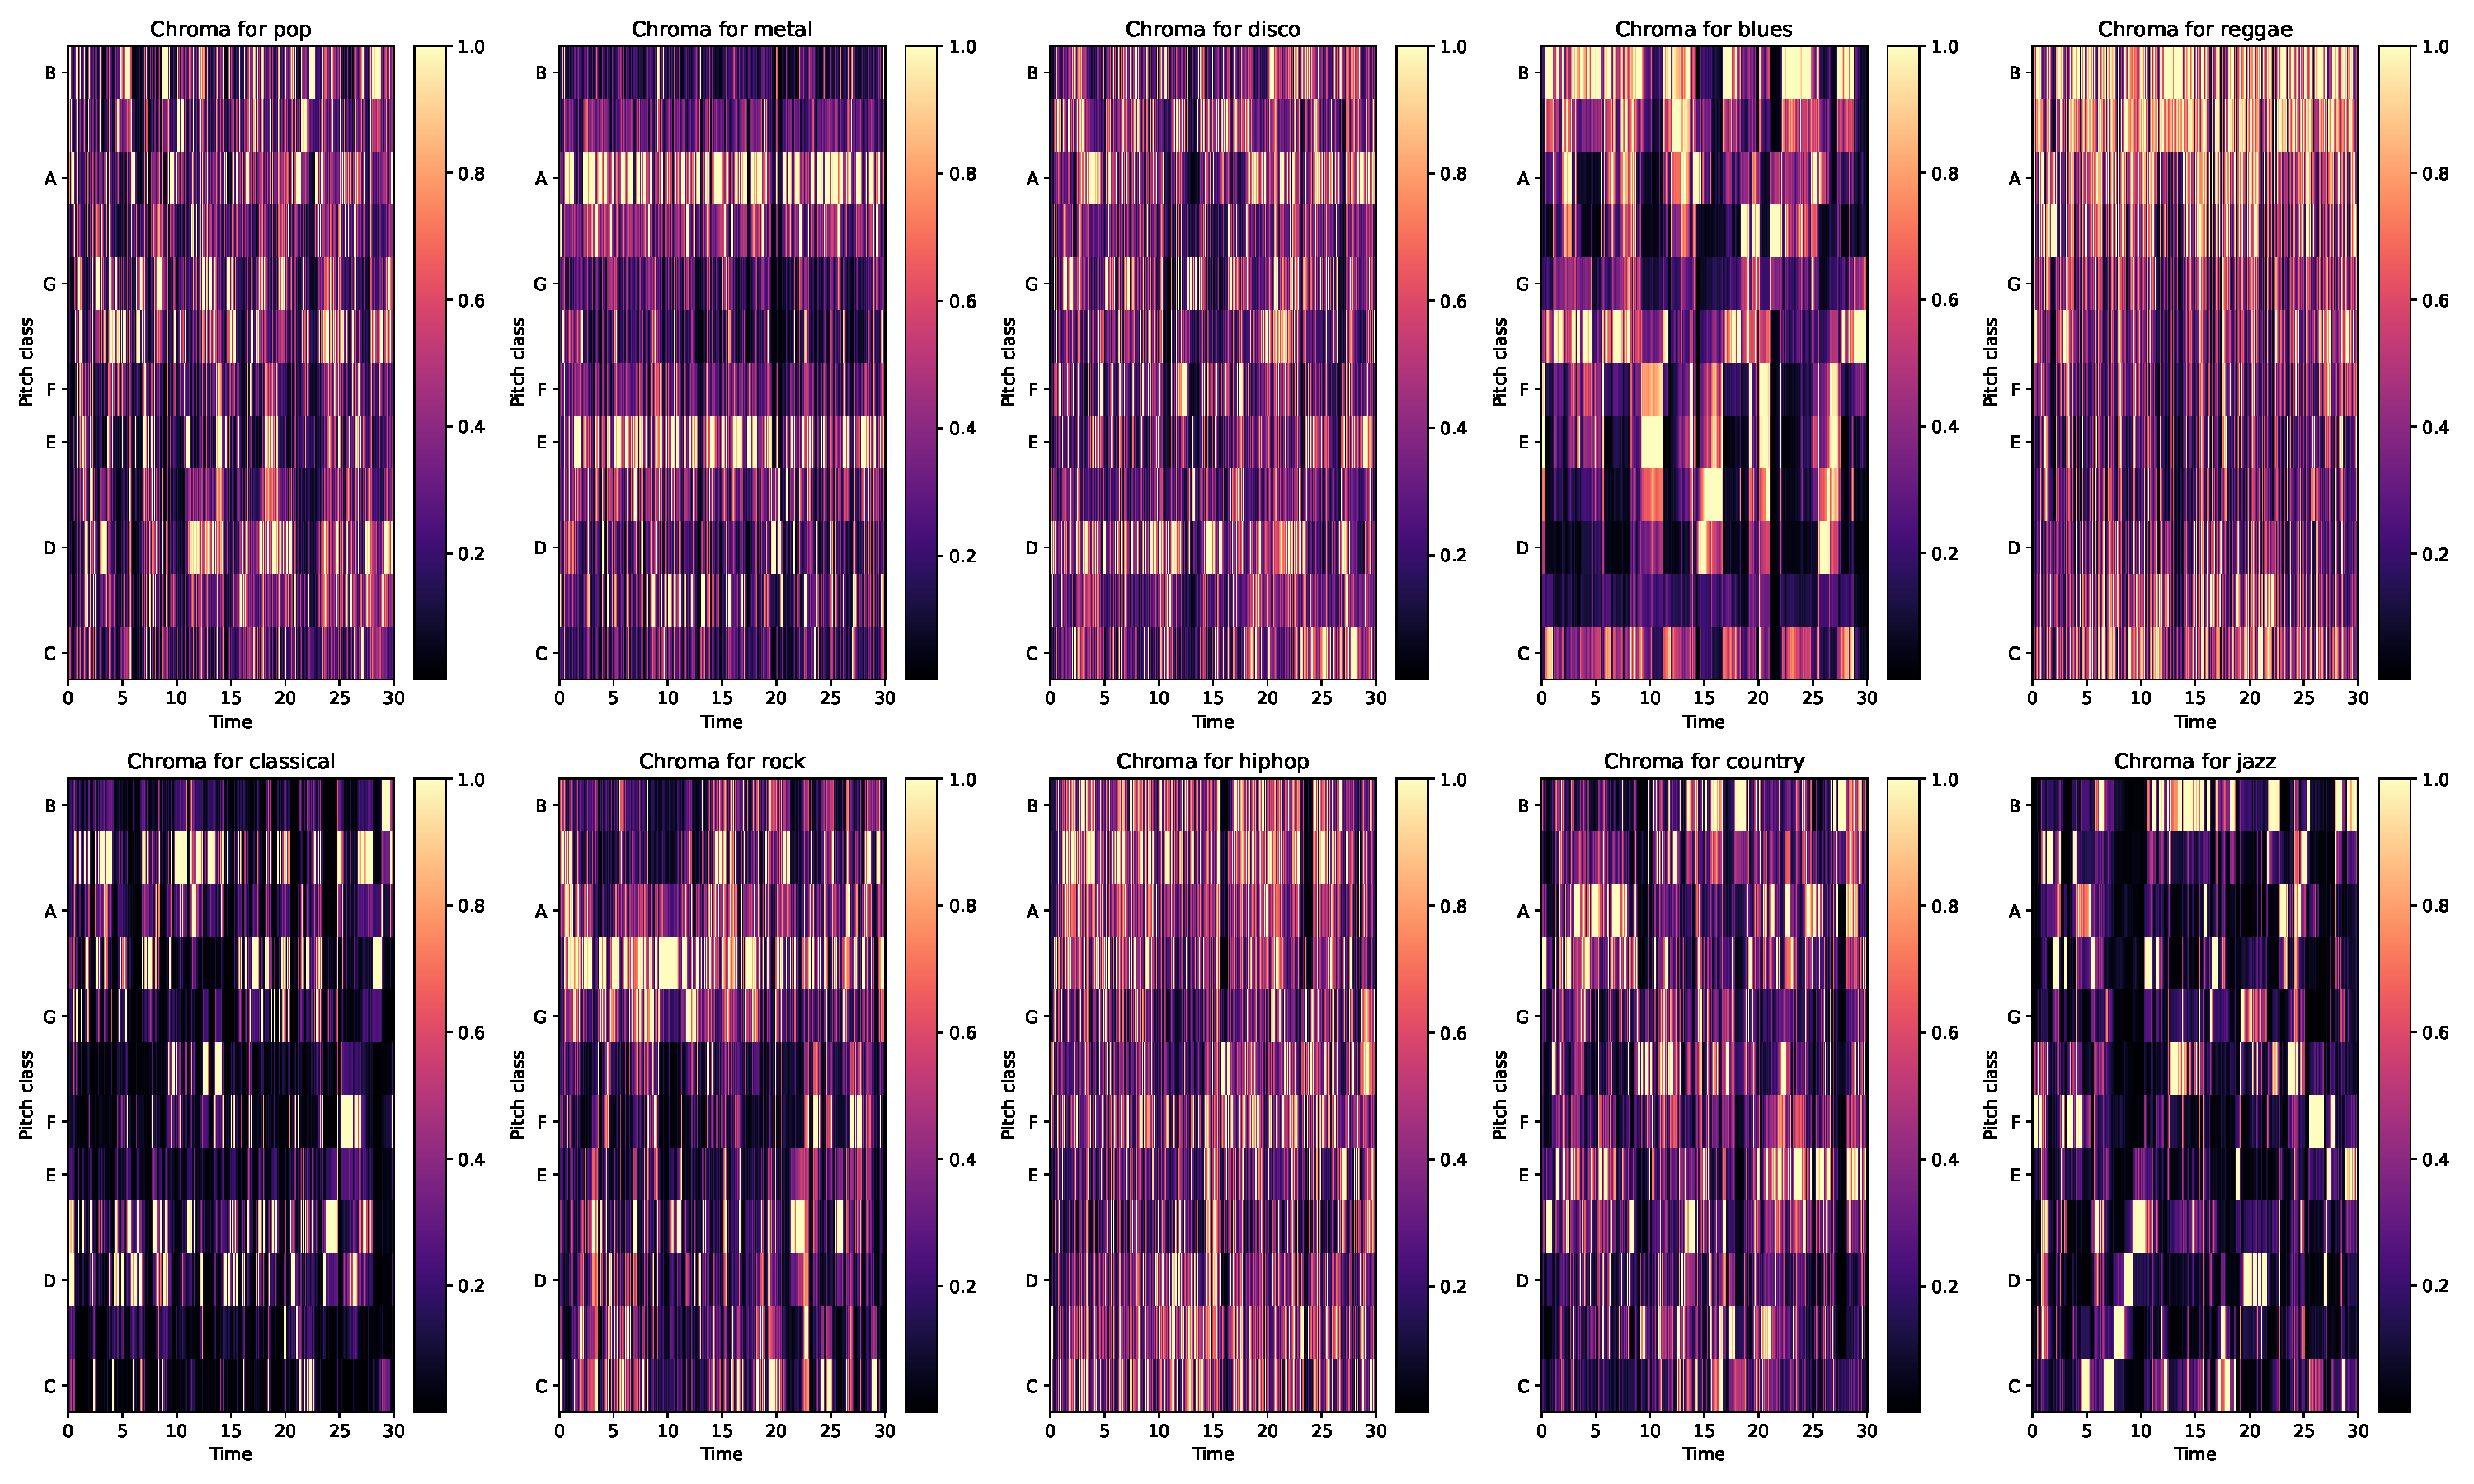
\includegraphics[width=0.75\textwidth]{images/chroma.pdf}
    \caption{Chroma Features of various pitch classes over time}
  \end{figure}
\end{frame}

\begin{frame}{Mel Spectrogram}
  \begin{figure}
    \centering
    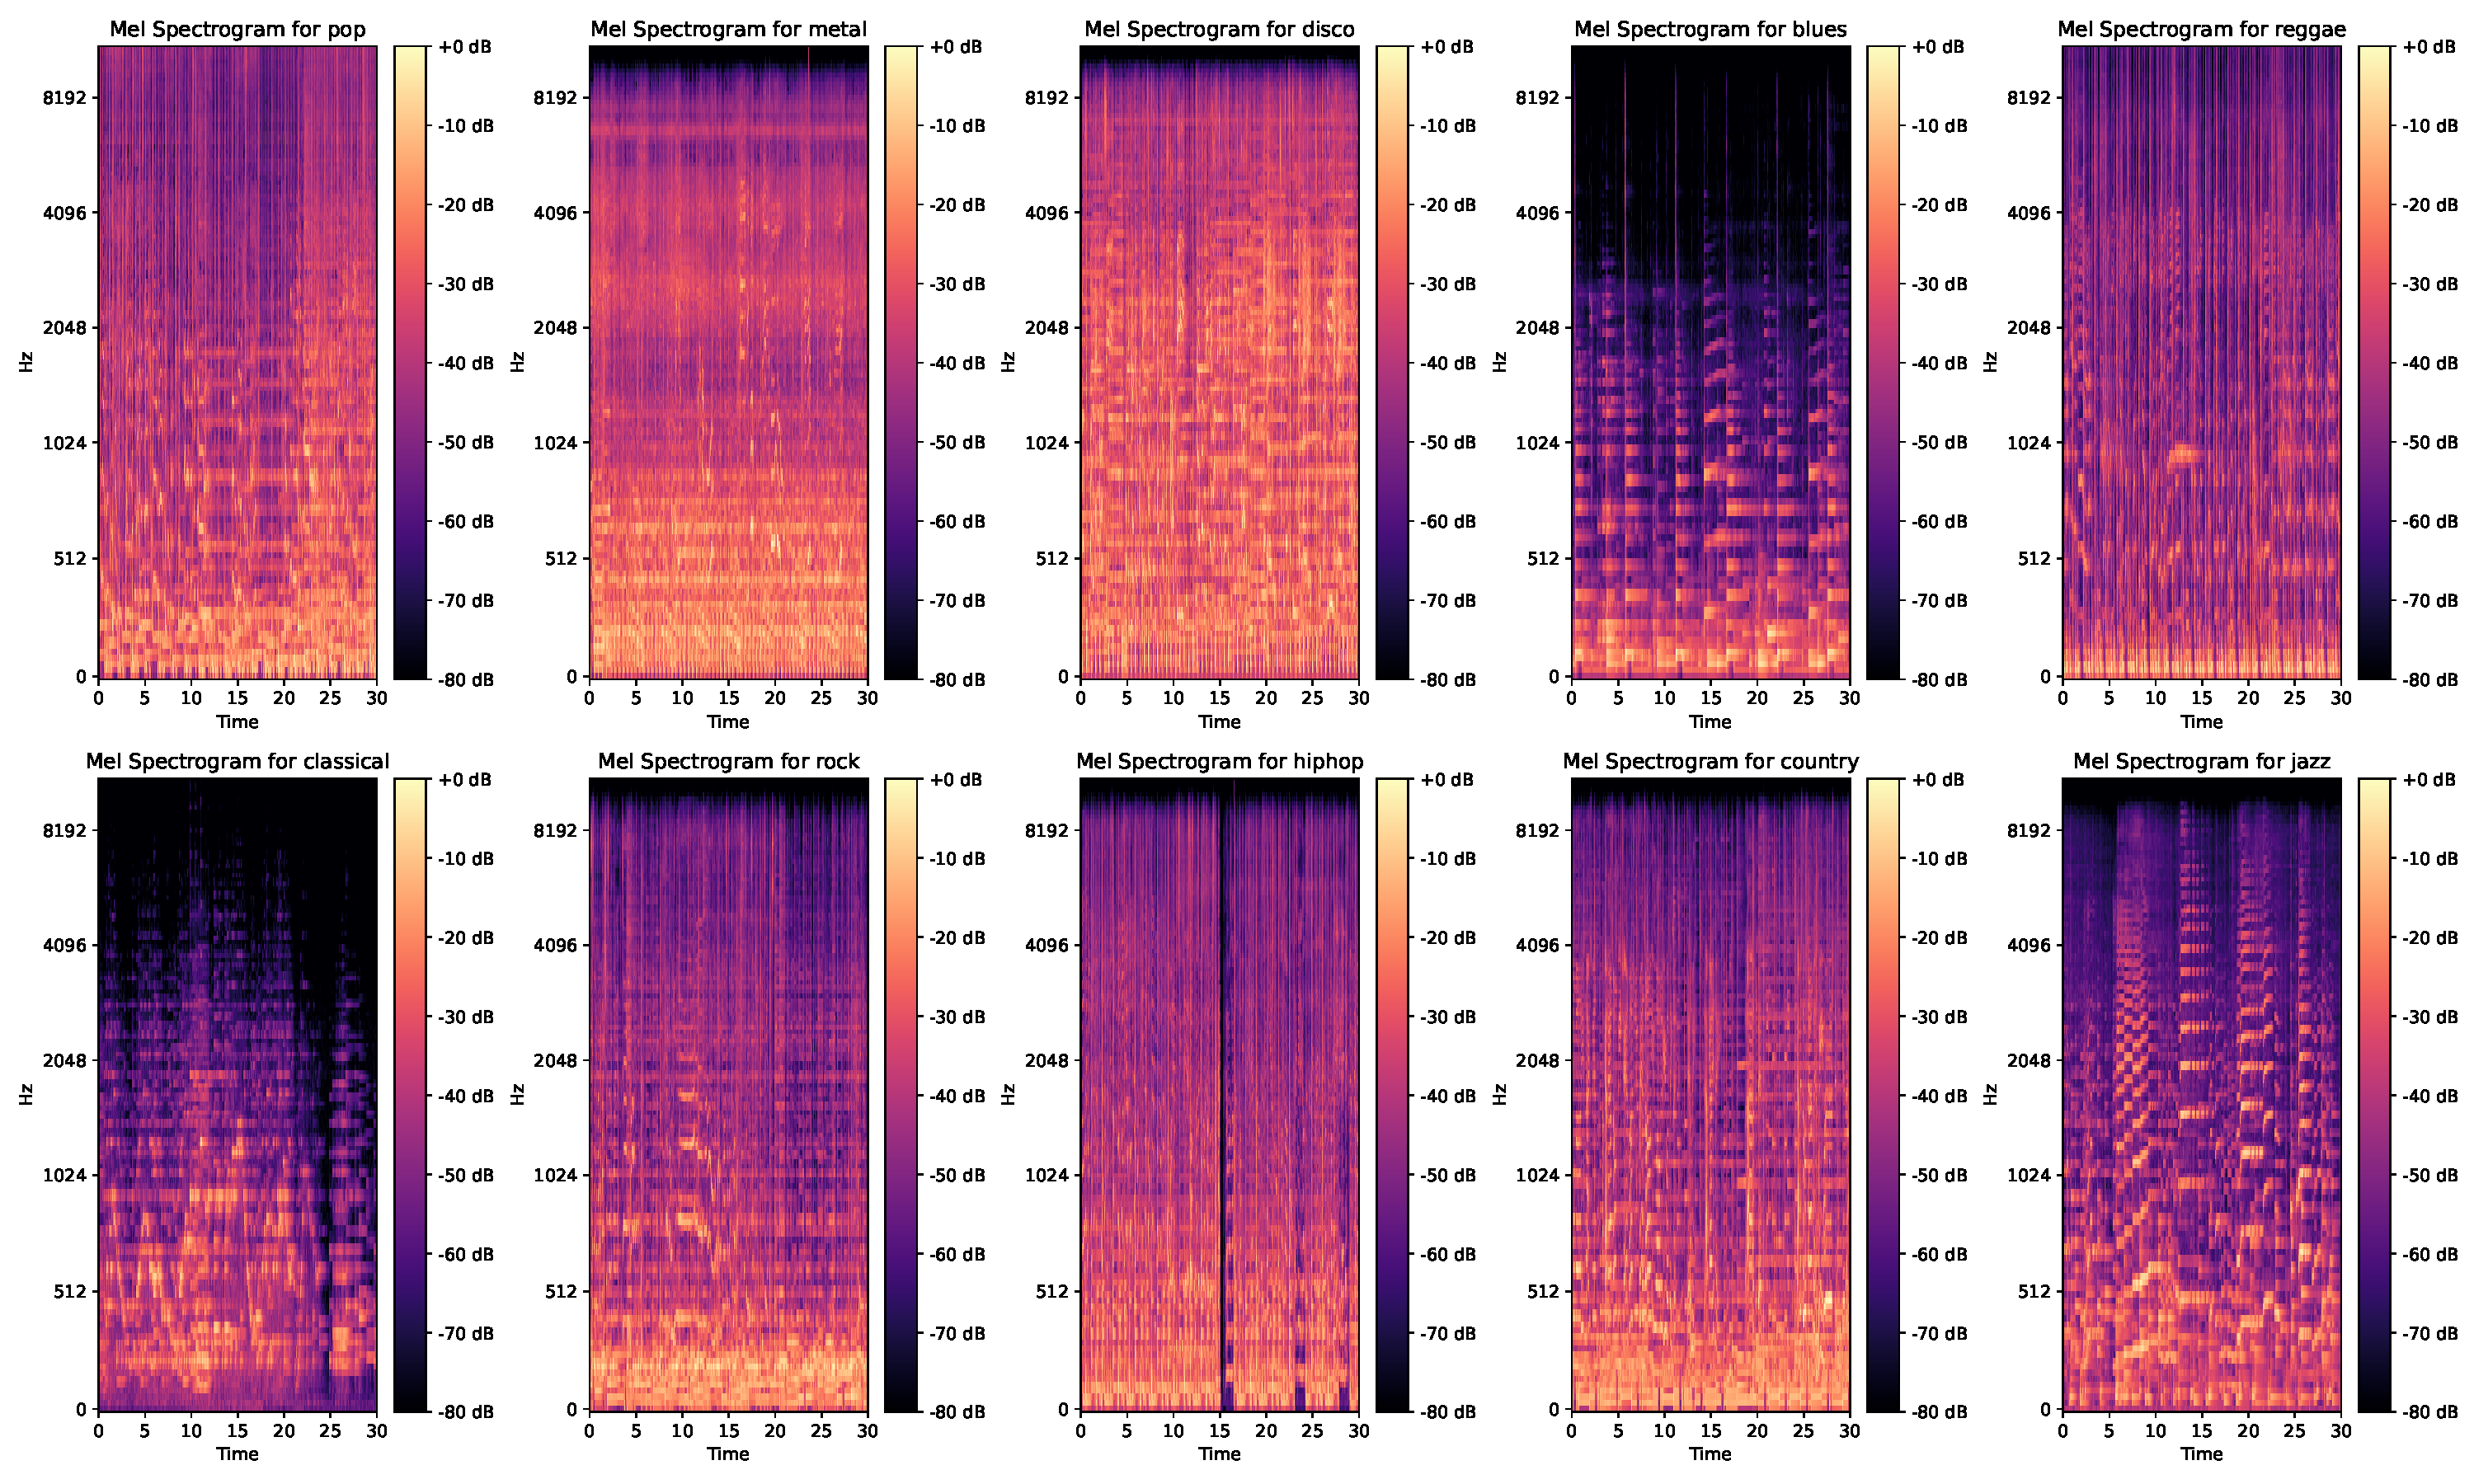
\includegraphics[width=0.75\textwidth]{images/mel.pdf}
    \caption{Mel Spectrogram of various sample audios track over time}
  \end{figure}
\end{frame}

\begin{frame}{Principal Component Analysis}
  \begin{figure}
    \centering
    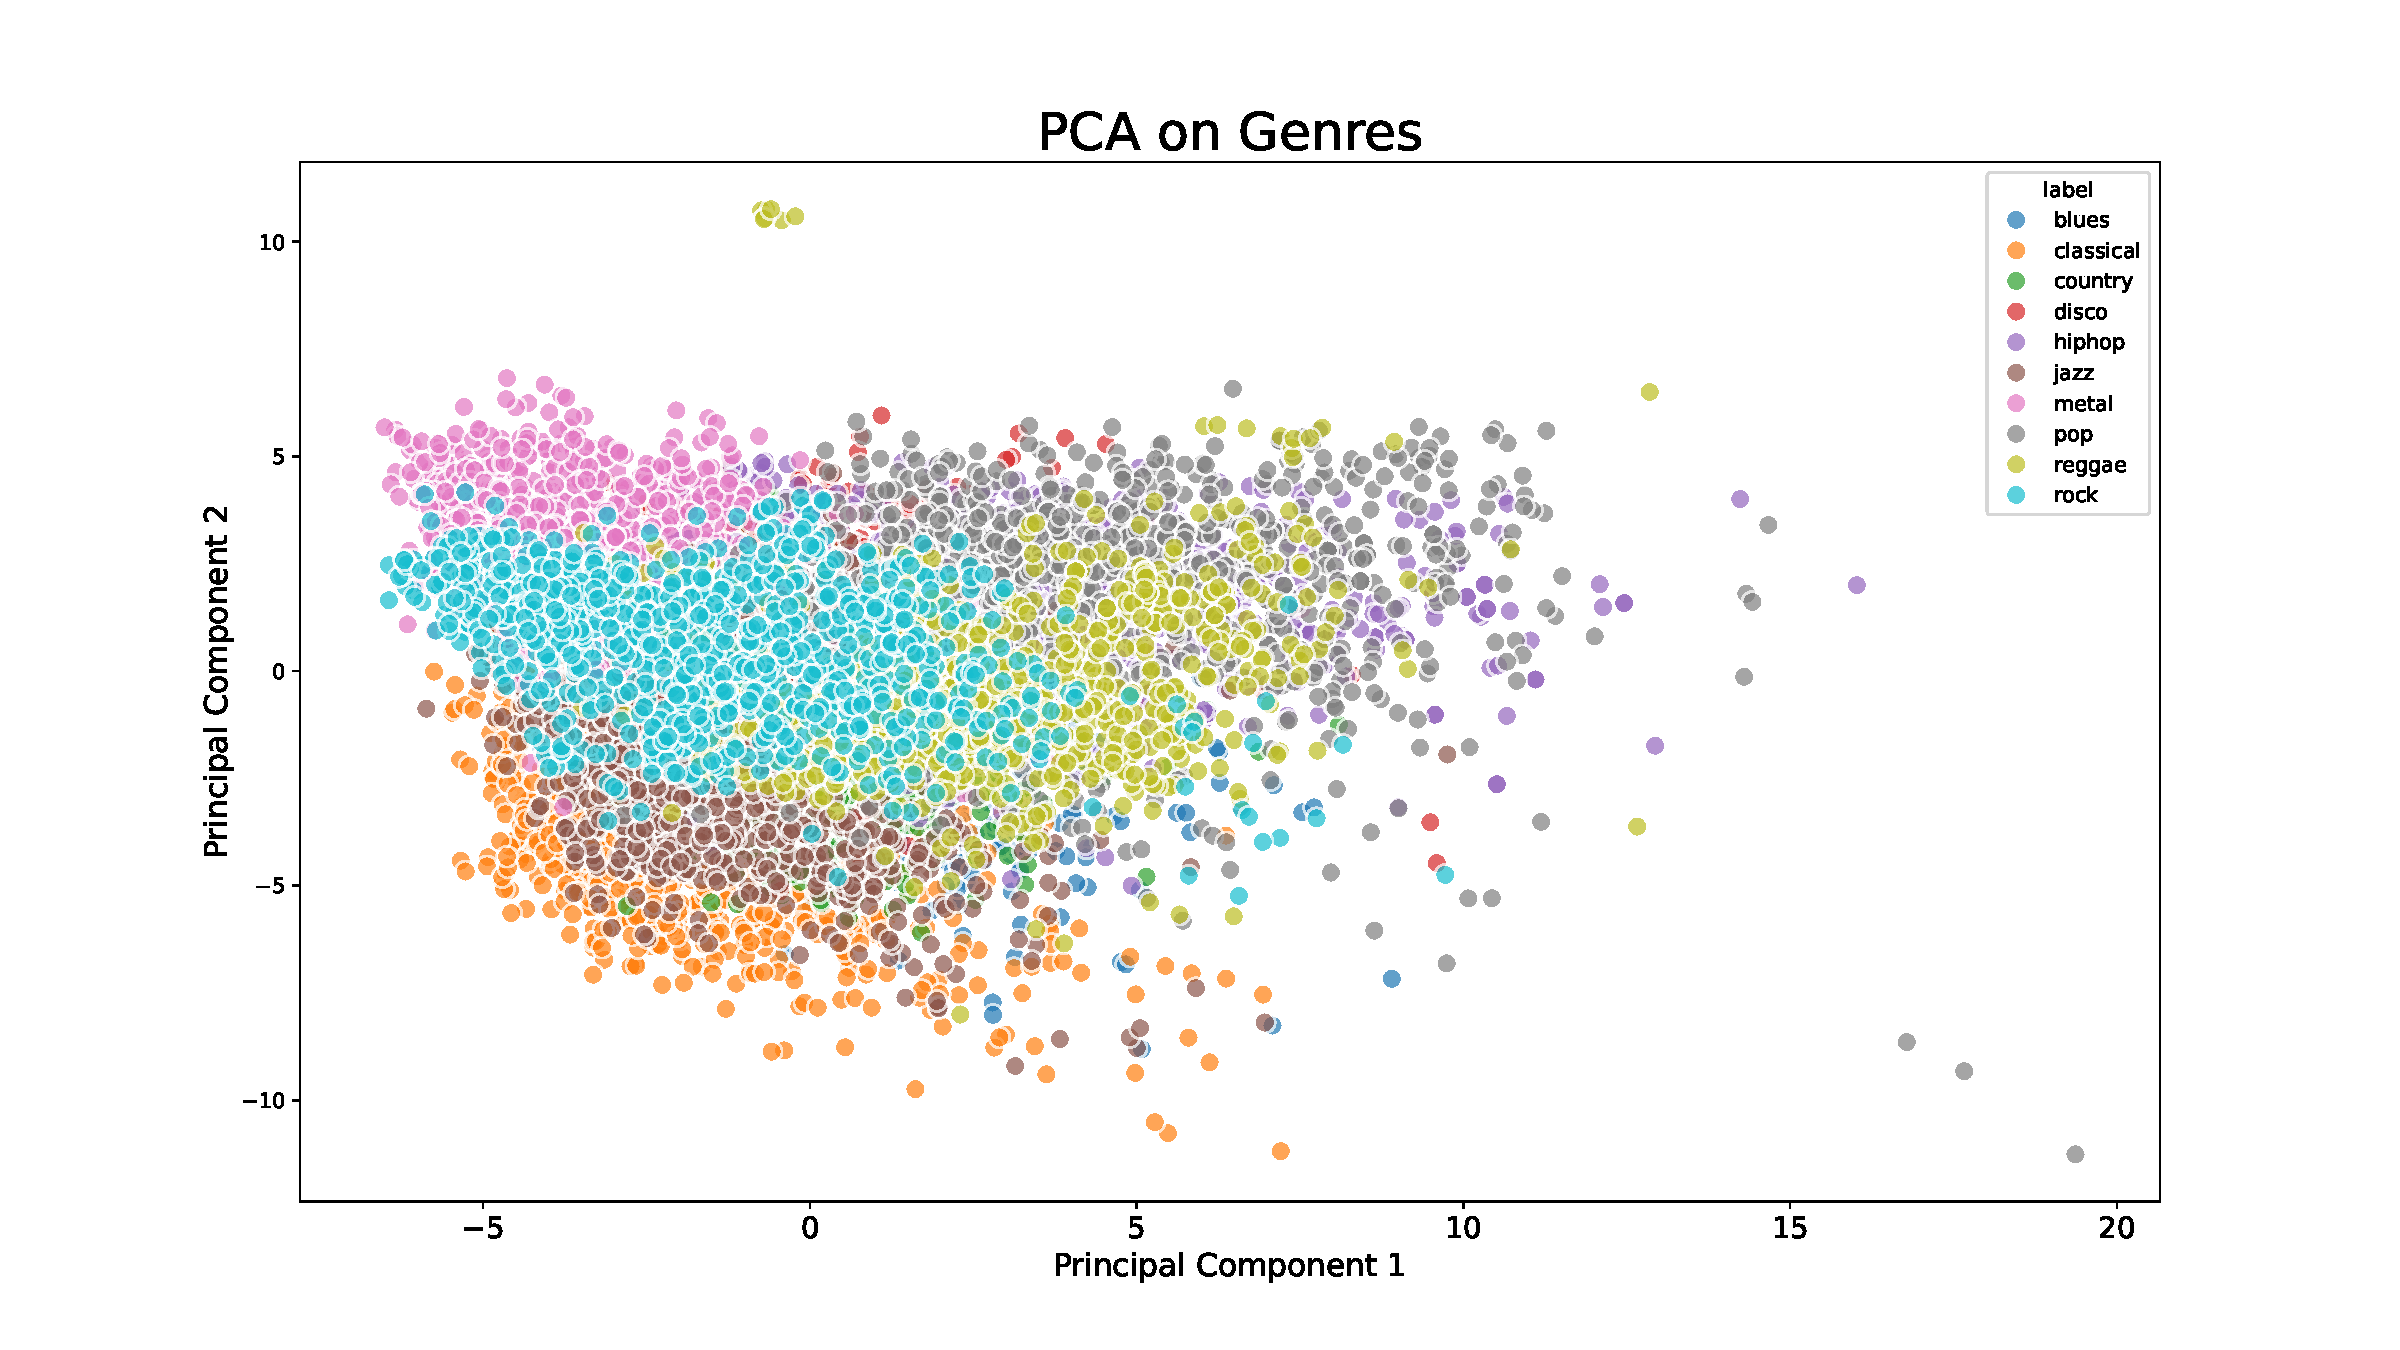
\includegraphics[width=0.8\textwidth]{images/pca.pdf}
    \caption{PCA of the GTZAN dataset}
  \end{figure}
\end{frame}

\section{Data Preprocessing}
\begin{frame}{Normalization}
  I used min-max scaling to normalize the features. The formula for min-max scaling is:
  \[ X_{norm} = \frac{X - X_{min}}{X_{max} - X_{min}} \]
\end{frame}

\begin{frame}{Data Splitting}
  I split the dataset into training and testing sets using an 8/2 split. And use 5-fold cross-validation to evaluate the models.
  \begin{figure}
    \centering
    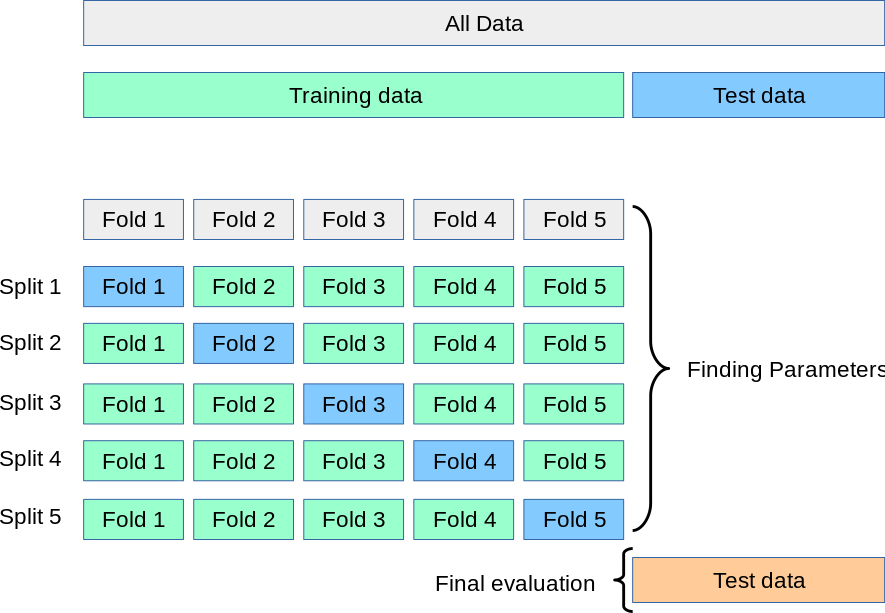
\includegraphics[width=0.5\textwidth]{images/grid_search_cross_validation.png}
    \caption{Data Splitting}
  \end{figure}
\end{frame}

\section{Machine Learning Models}
\begin{frame}{Baseline Models}
  I trained several traditional machine learning models on the dataset to establish a baseline performance. The models I used are:
  \begin{itemize}
    \item Logistic Regression
    \item Support Vector Machine
    \item  Decision Tree
    \item Logistic Regression
    \item Random Forest
    \item XGBoost
  \end{itemize}
\end{frame}

\begin{frame}{Baseline Models}
  The results on the training set are summarized in figure, with the x-axis representing \textbf{accuracy}. The XGBoost model outperformed the other models, achieving an accuracy of 0.91 on the training set.

  \begin{figure}
    \centering
    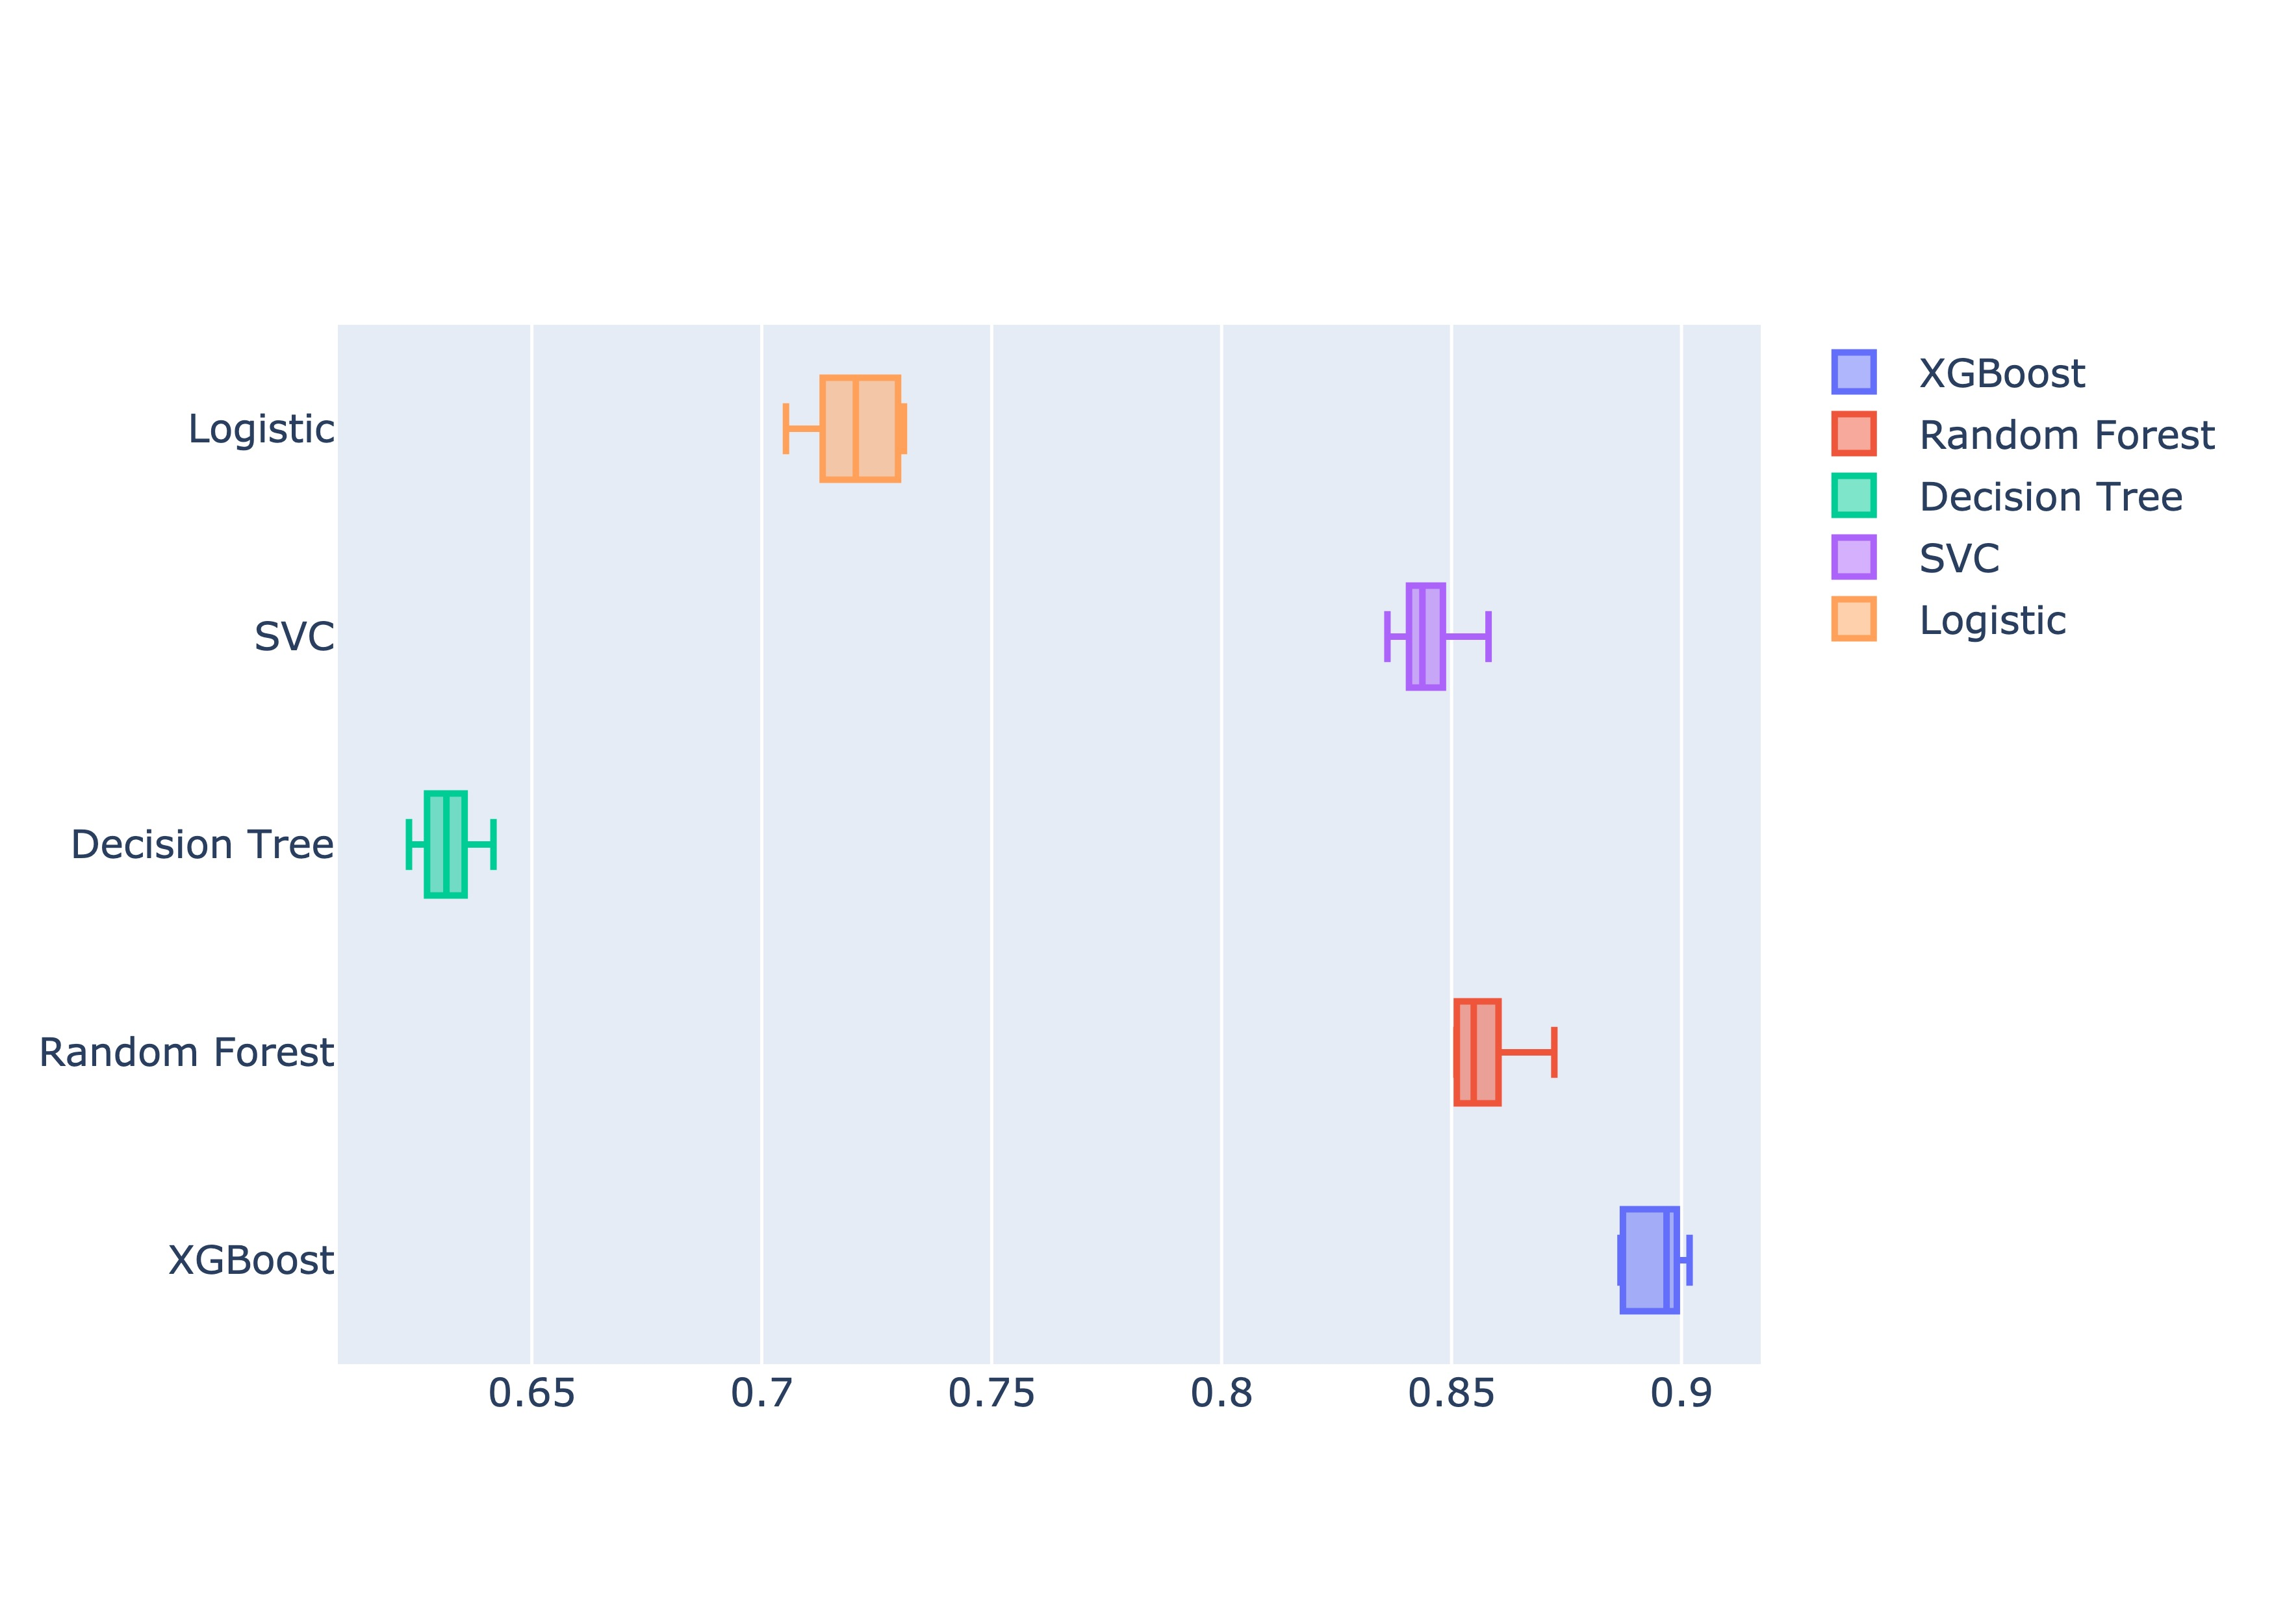
\includegraphics[width=0.5\textwidth, trim=0pt 140pt 0pt 140pt, clip]{images/baseline_models.jpg}
    \caption{Baseline Models}
  \end{figure}
\end{frame}

\begin{frame}{Model Evaluation}
  I evaluated the XGBoost model on the testing set and obtained an accuracy of 0.90. The confusion matrix in figure shows that the model performs well for some genres (e.g., classical, metal) but struggles with others (e.g., rock, country).

  \begin{figure}
    \centering
    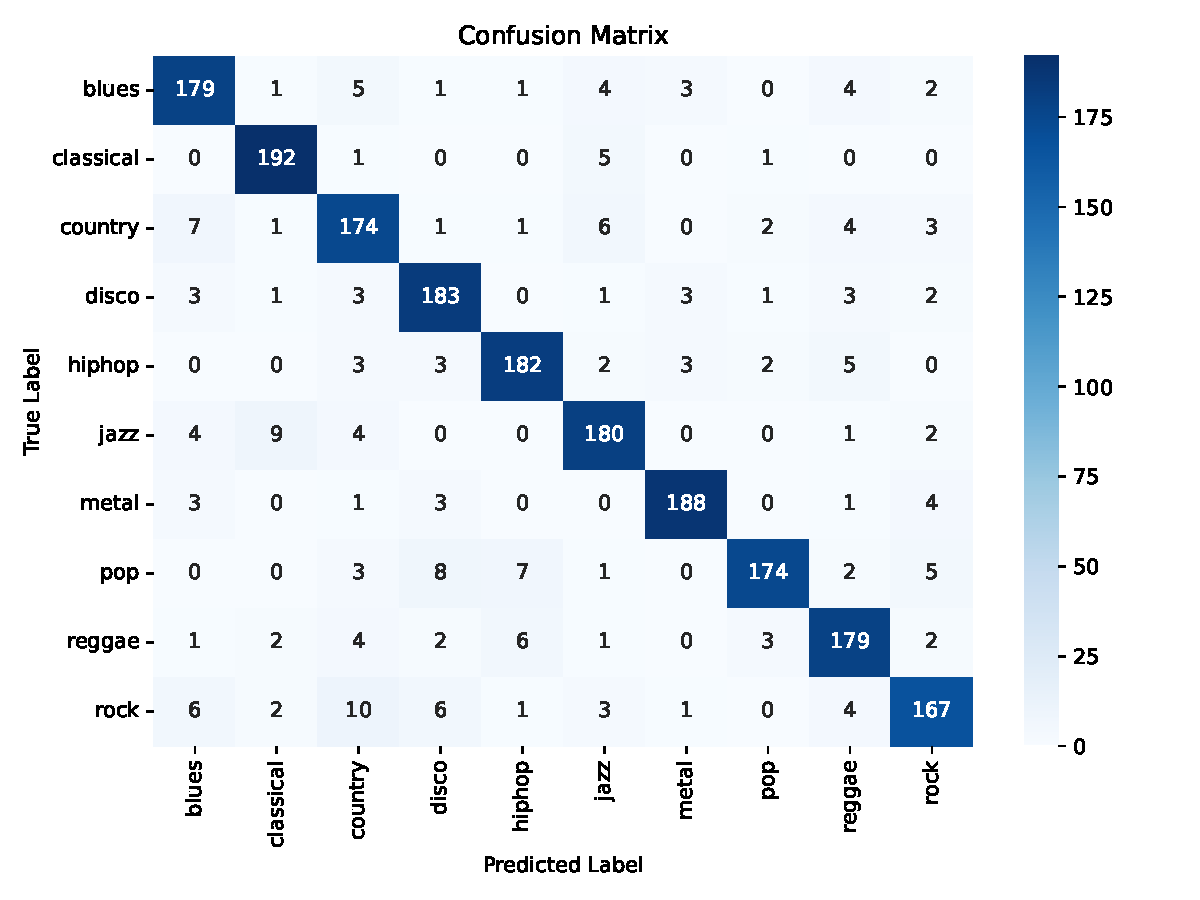
\includegraphics[height=0.4\textwidth]{images/confusion_matrix.pdf}
  \end{figure}
\end{frame}

\begin{frame}{Model Evaluation}
  \begin{figure}
    \centering
    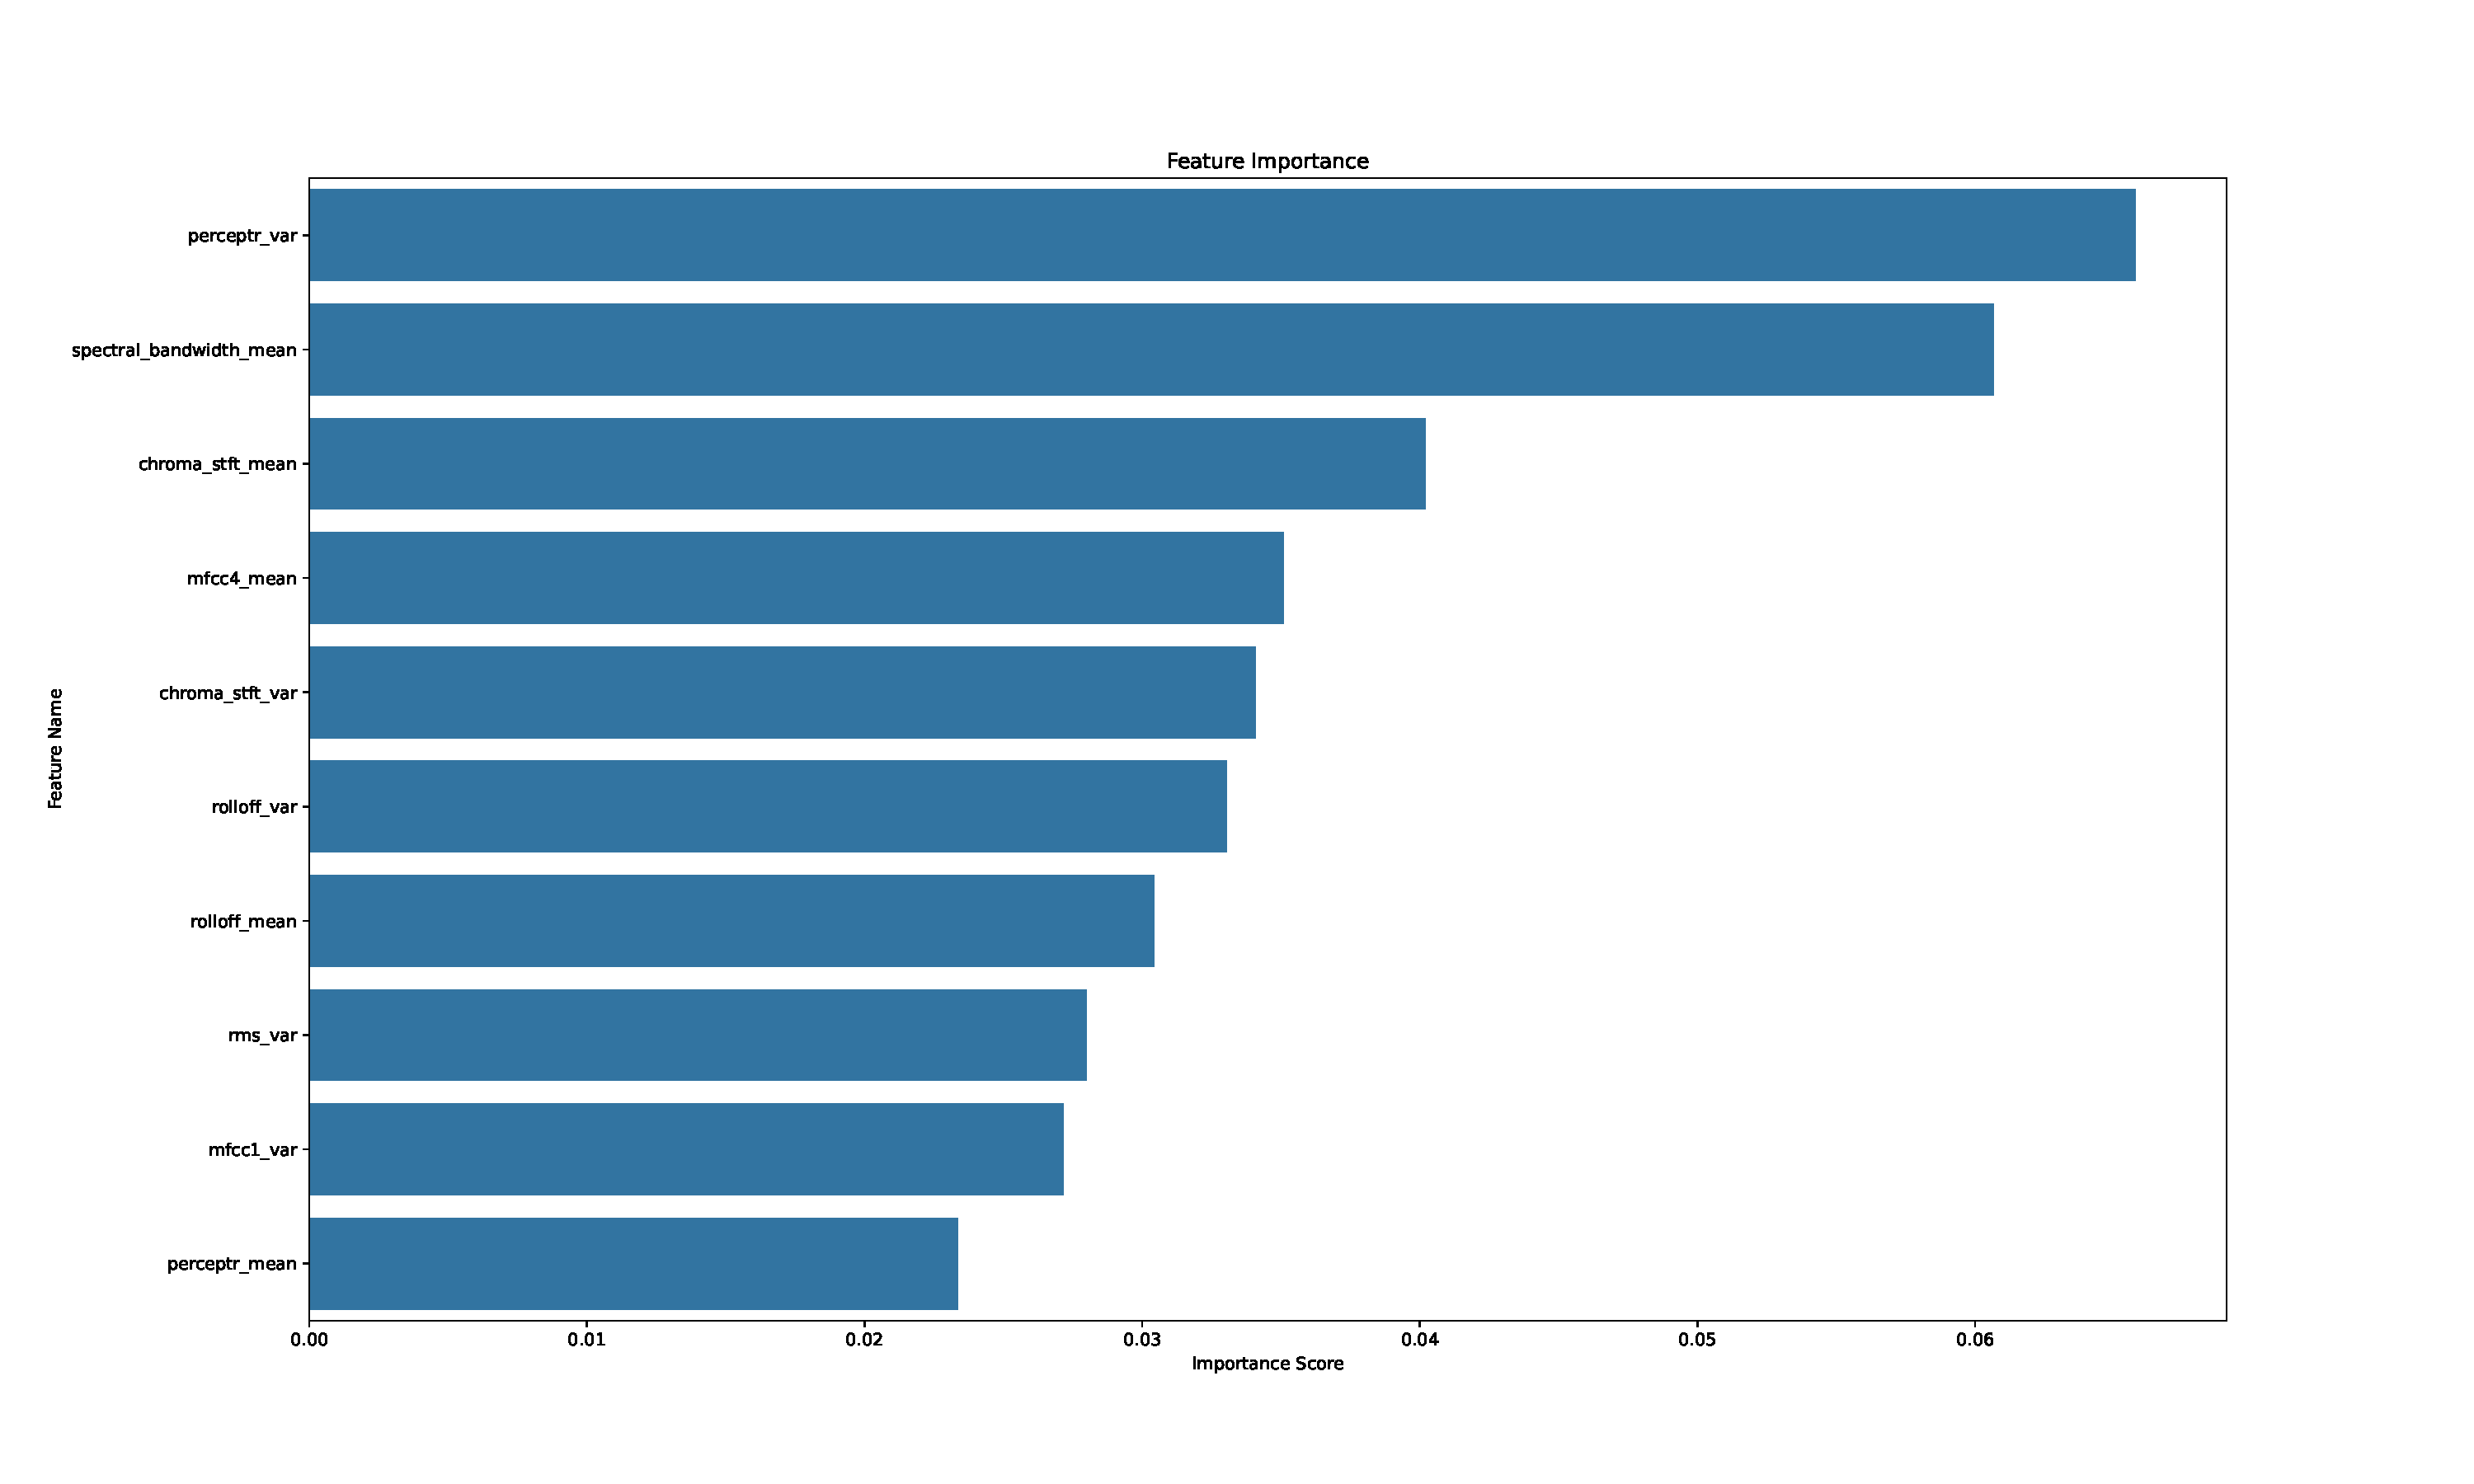
\includegraphics[height=0.5\textwidth]{images/feature_importance.pdf}
  \end{figure}
\end{frame}

\begin{frame}{Hyperparameter Tuning}
  I used \textbf{RandomizedSearchCV} to tune the hyperparameters of the XGBoost model. The best hyperparameters found by RandomizedSearchCV were:
  \begin{itemize}
    \item n\_estimators: 100
    \item max\_depth: 3
    \item learning\_rate: 0.1
    \item subsample: 0.8
    \item colsample\_bytree: 0.8
  \end{itemize}
\end{frame}

\section{Convolutional Neural Network (CNN)}
\begin{frame}{Model Architecture}
  The CNN architecture consists of five convolutional layers followed by max pooling layers and two fully connected layers. The model is trained on the mel spectrogram of the audio tracks.
\end{frame}

\begin{frame}{Model Architecture}
  \begin{figure}
    \centering
    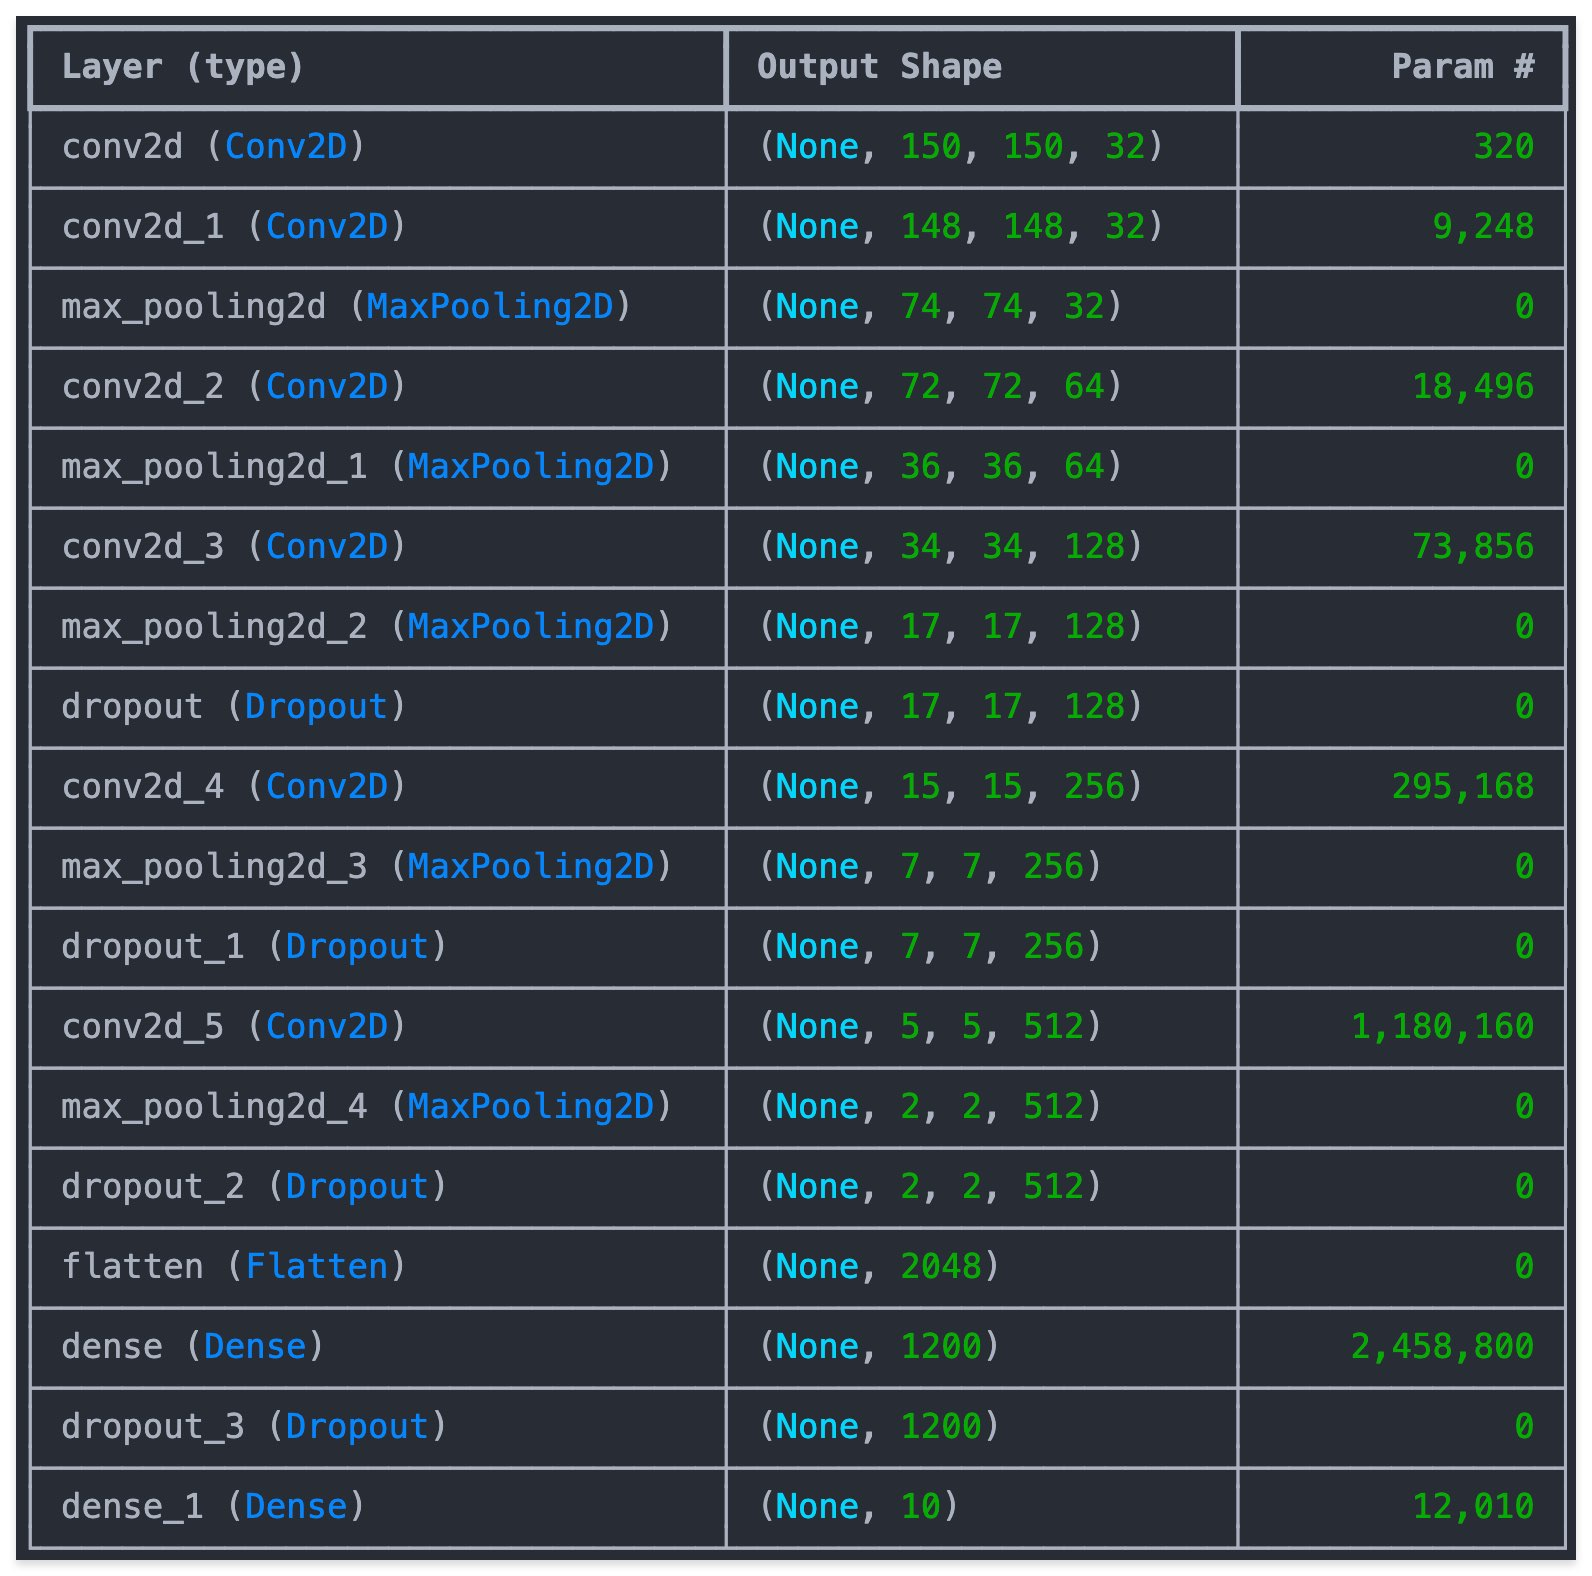
\includegraphics[width=0.5\textwidth]{images/model_architecture.jpg}
  \end{figure}
\end{frame}

\begin{frame}{Model Training}
  The figure illustrates a decreasing loss and increasing accuracy over time, indicating effective learning. However, as the number of epochs increases, there is a risk of \textbf{overfitting}.
  \begin{figure}
    \centering
    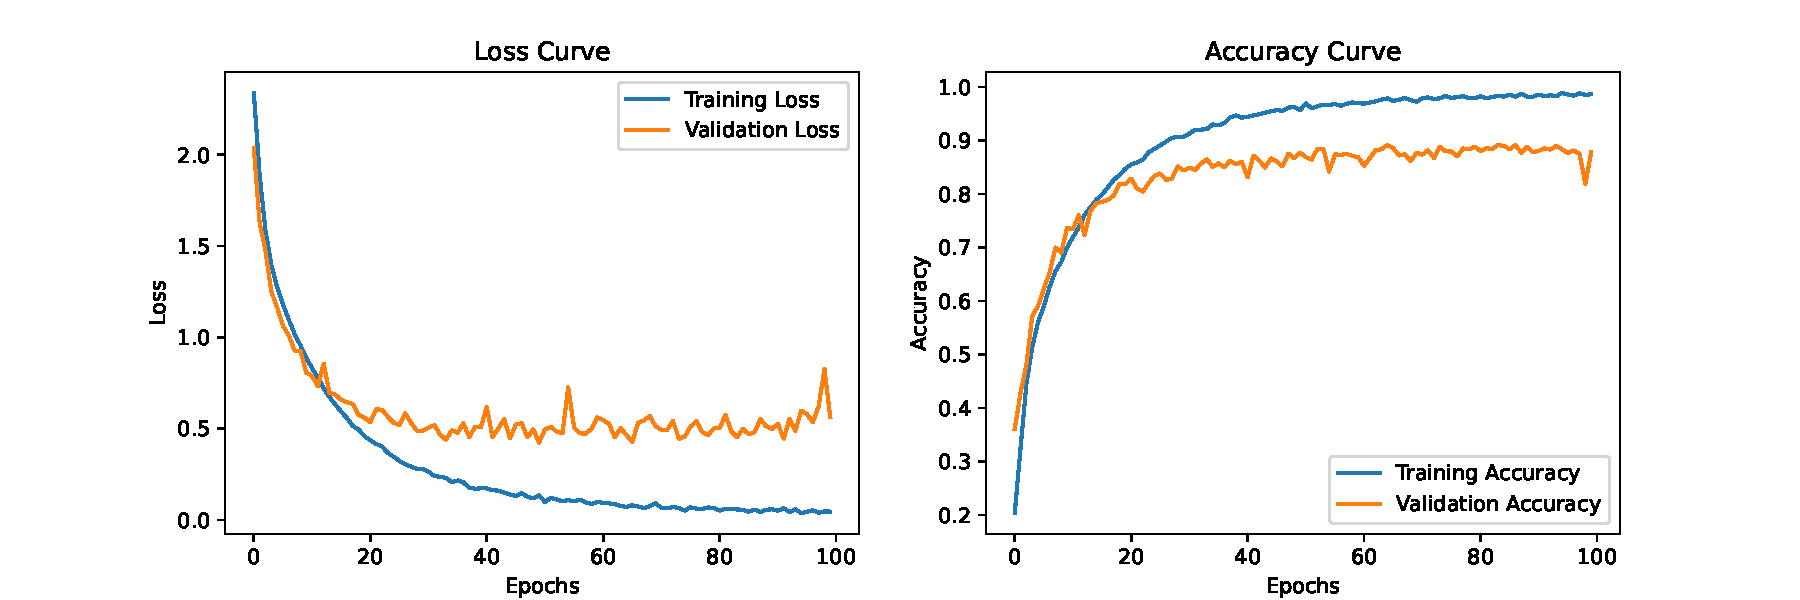
\includegraphics[width=0.9\textwidth]{images/loss_accuracy.pdf}
    \caption{Loss and Accuracy Curves during training}
    \label{fig:loss_accuracy}
  \end{figure}
\end{frame}

\begin{frame}{Model Evaluation}
  It achieved an accuracy of 0.87 on the testing set. The confusion matrix in figure indicates that the CNN model performs well for most genres. However, it encounters difficulties with genres like jazz and reggae, which exhibit similar spectral characteristics.
  \begin{figure}
    \centering
    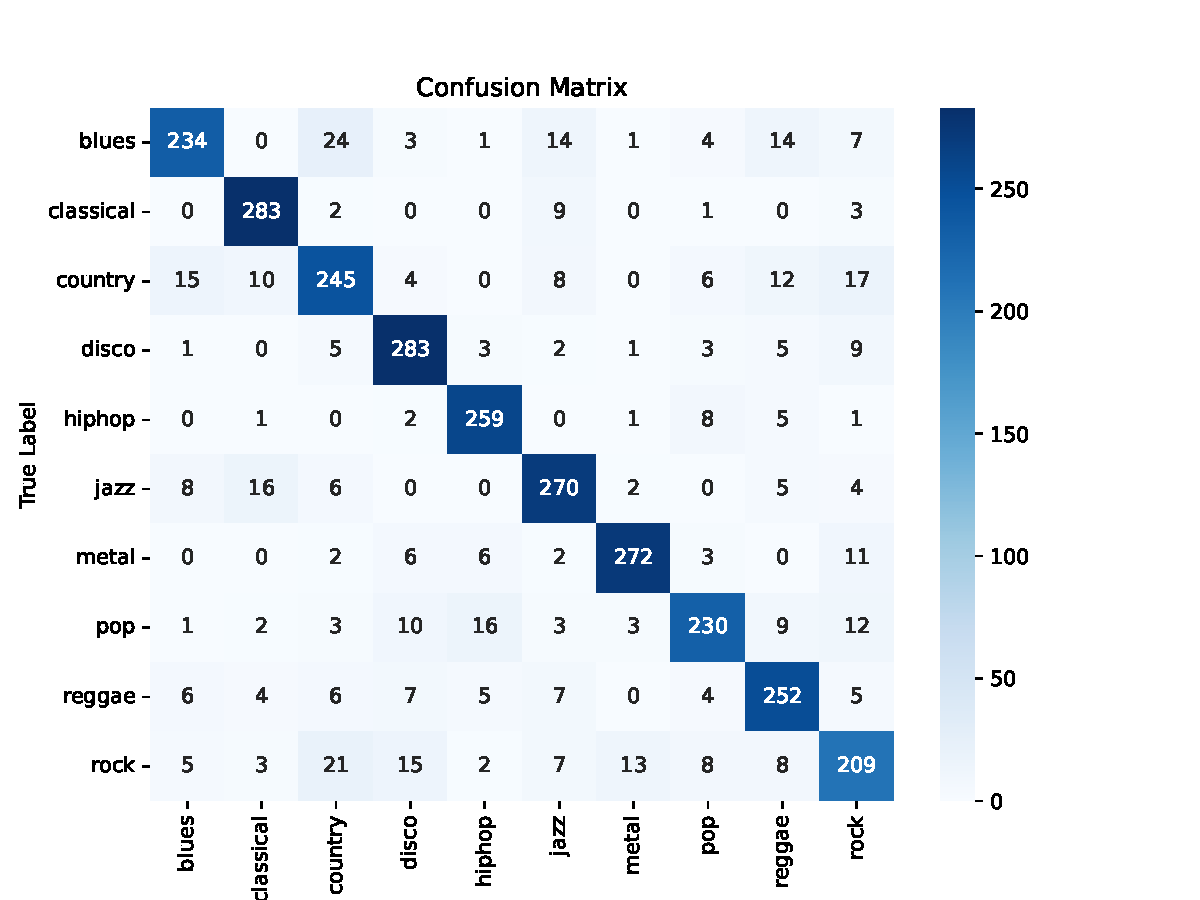
\includegraphics[height=0.4\textwidth]{images/cnn_evaluation.pdf}
  \end{figure}
\end{frame}

\section{Conclusion}
\begin{frame}{Conclusion}
  It is evident that XGBoost is the most suitable model for this classification task. The CNN model underperformed compared to traditional models because CNNs are optimized for spatial data.

  Traditional models like SVC and XGBoost utilize manually extracted features (such as MFCC, Chroma, Spectral Contrast, Zero-Crossing Rate, etc.) that are specifically designed to capture audio patterns effectively.

  \begin{table}[h]
    \centering
    \begin{tabular}{ccccc}
      \toprule
      \textbf{Model} & \textbf{Accuracy} & \textbf{Precision} & \textbf{Recall} & \textbf{F1\-score} \\
      \midrule
      SVC            & 0.85              & 0.85               & 0.85            & 0.85               \\
      Random Forest  & 0.87              & 0.87               & 0.87            & 0.87               \\
      CNN            & 0.87              & 0.87               & 0.87            & 0.87               \\
      XGBoost        & 0.91              & 0.91               & 0.91            & 0.91               \\
      \bottomrule
    \end{tabular}
    \caption{Model Performance on testing set}
    \label{tab:performance}
  \end{table}
\end{frame}
\end{document}
